\begin{figure}
    \centering
    \subfloat[Cophylogeny of gophers and lice]{%
        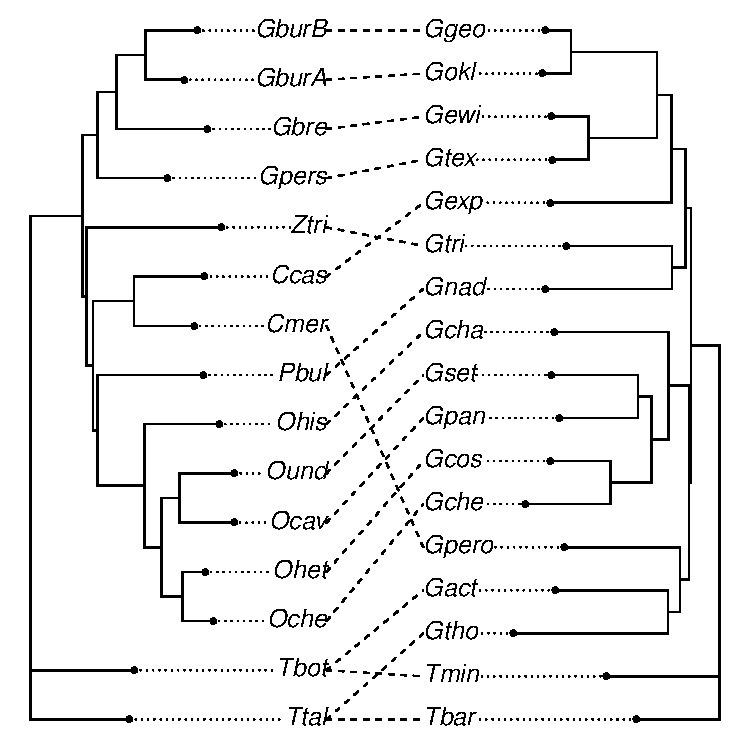
\includegraphics[width=0.5\textwidth]{figures/gopher_louse_cophylo}
    }
    \subfloat[Paired patristic distances]{%
        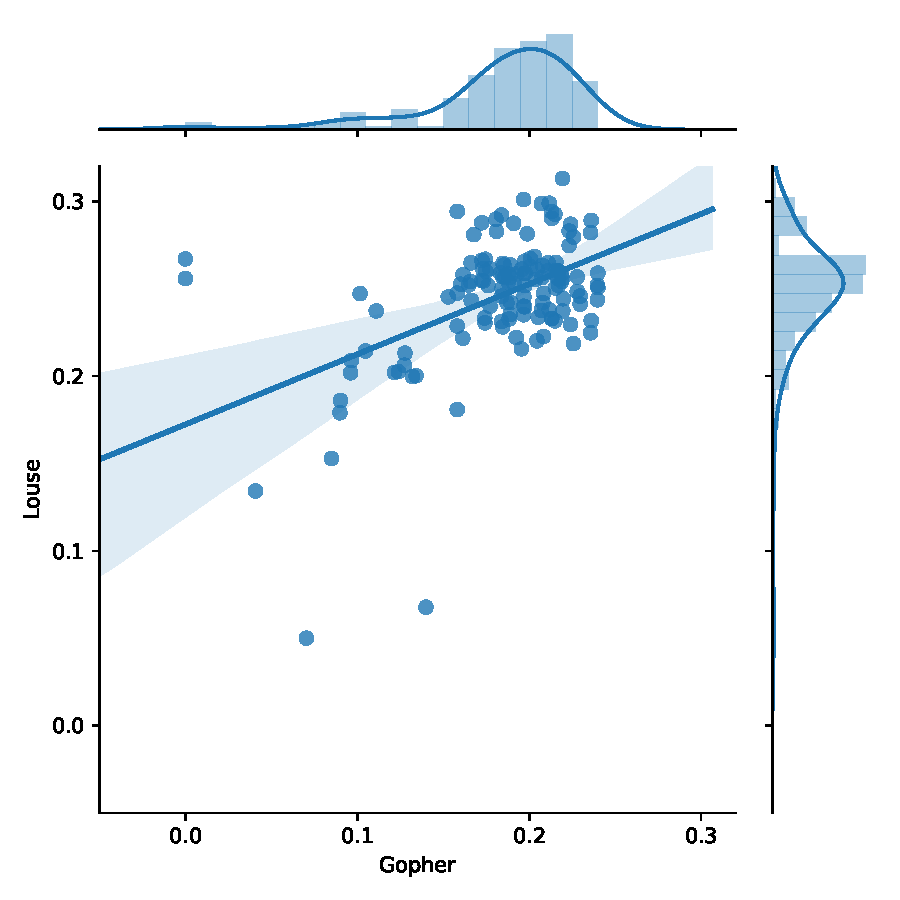
\includegraphics[width=0.5\textwidth]{figures/gopher_louse_correlation}
    }
    \caption{The relationship between pocket gophers and their chewing lice parasites has served as a benchmark case in the literature on coevolution since its appearance in Hafner {\em et al.} \cite{hafner1994disparate}. However, despite the strong case for coevolution from multiple lines of evidence, the agreement between the two trees (as measured by the correlation of pairwise patristic distances through the two trees \cite{hommola2009permutation}) is modest, with a Pierson's $r$ of 0.49. If one were to exclude the relationships between the outgroups as outliers, the correlation would collapse. Without other forms of evidence, the detection of such relationships is challenging.}
    \label{fig:gopher-louse}
\end{figure}
